\chapter{Introduction}

\section{Motivation}

%Traditionally, motor learning needs a from of instruction and a student willing to learn a motor skill. For example in a dance lesson, a teacher stands in front of one or more students performing a movement and the student's are watching this demonstration followed by mimicking the movement on their own. 
%heranführung zum thema, erklären warum das wichtig ist.
In recent years, Mixed Reality (MR) devices became affordable\footnote{\hyperlink{https://www.vive.com/}{vive.com}, \hyperlink{https://www.oculus.com/}{oculus.com}accessed: 3.12.2019}, portable\footnote{\hyperlink{https://arvr.google.com/daydream/}{arvr.google.com/daydream} accessed: 3.12.2019} and usable in many conditions. Not only academic researchers are interested in this technology, but commercial companies also found MR devices helpful to explore new possibilities to use them profitably. With this development, learning and training in MR became possible for many cases, too. EON\footnote{\hyperlink{https://www.eonreality.com/}{https://www.eonreality.com/} accessed: 14.12.2018}, for example, calls themself "the world leader in Virtual Reality based knowledge transfer for industry, education, and edutainment". They develop MR programs for several platforms, e.g. intending to guide workers, reducing mistakes and thus reducing costs. These programs address a lot of use cases in the field of education, energy, health \& medical, manufacturing \& industrial, defence \& security and aerospace. Tasks include e.g. ground crew training for a Boeing 777, augmented reality (AR) assembly training, exploring or anatomy simulation, to mention only a few.\\
Microsoft also stepped into this topic with partners, developing tools for apprenticeship, maintenance, or remote training. E.g. The Smart Glass experience Lab\footnote{\hyperlink{https://www.fit.fraunhofer.de/de/fb/cscw/smart-glasses-experience-lab.html}{fit.fraunhofer.de/de/fb/cscw/smart-glasses-experience-lab.html} accessed: 18.11.2019} of the Fraunhofer Institute use the MS Hololens\footnote{\hyperlink{https://www.microsoft.com/en-us/hololens}{microsoft.com/en-us/hololens} accessed: 3.12.2019} for remote maintenance, compare figure~\ref{fig:fraunhofer}.
\begin{figure}
	\centering
	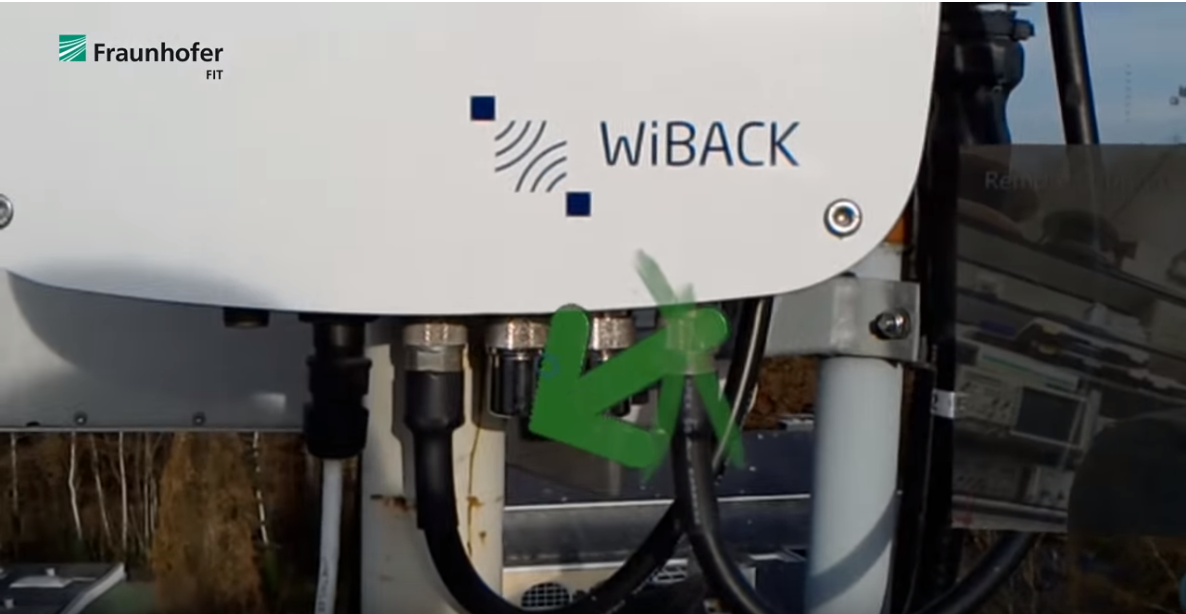
\includegraphics[width=1.0\textwidth]{img/fraunhofer.PNG}
	\caption{Remote maintenance with Hololens by Smart Glass Experience Lab. The on-site worker wears a Hololens, while the remote trainer draws green hints to resolve a miss-wiring, taken from \hyperlink{https://www.youtube.com/watch?v=1QFMPo5k6p0}{https://www.youtube.com/ watch?v=1QFMPo5k6p0}, accessed (30.07.2019)}
	\label{fig:fraunhofer}
\end{figure}\\
Motor learning plays a mayor role in our everyday life when it comes to \--- for example \--- sports, arts or dancing. Gaining proficiency in one of these areas is not possible without intense motor learning. Mostly a teacher or trainer is required for progress. For example, a student wants to learn a movement from a teacher. In the real world, the teacher stands in front of the student performing the movement and the student tries to mimic it. This visual perspective is called exo-centric or 3rd person perspective. If for example, a teacher is not available or affordable, other sources for motor learning are available like videos. Still, these videos are in the exo-centric perspective. But, with today's MR technology we have the possibility to change this perspective what we cannot do in the real world. A student can "step into" the teacher's virtual body and see the instruction from the 1st person perspective of the teacher, also called ego-centric perspective. For developing MR learning and training environments, researchers put much effort into developing how-to's and guidelines to ensure proper systems e.g. \cite{LaViola2017}. However - as we will see in chapter 3 - there is a research gap about the visual perspective in these systems. The implication of the change of the visual perspective is not investigated sufficiently. This work aims to close this gap. 
This seminar thesis is the first out of three parts, followed by a master's project and a master's thesis. The overall aim of this work is to answer the following main research question:
\begin{itemize}
	\item[MRQ] Does the visual perspective on a virtual guidance visualisation have an influence on motor learning in MR environments.
\end{itemize}
The answer to this research question is important for designing motor learning systems for mixed reality.\\
The outcome of this work is a study design that will be able to address the research questions. In the master's project, the proposed study will be implemented. With this system a study will be conducted, generating the data to answer the research question. The master's thesis itself will take the generated data to finally answer the research question.


\section{Outline}
For a well-developed study design, many aspects must be taken into consideration. The main aspects will be discussed in this work. Further aspects like algorithms and technology are discussed in the master's project. In chapter 2 this work sets the scope and provides theoretical foundations. in chapter 3 the parameters for the study design are discussed utilizing related work. With the scope and parameters set, chapter 4 proposes a study design which serves as the base for the master's project. In the end, an outlook on the master's project and master's thesis is given. Compare figure~\ref{fig:overallProcess}.
\begin{figure}[h]
	\centering
	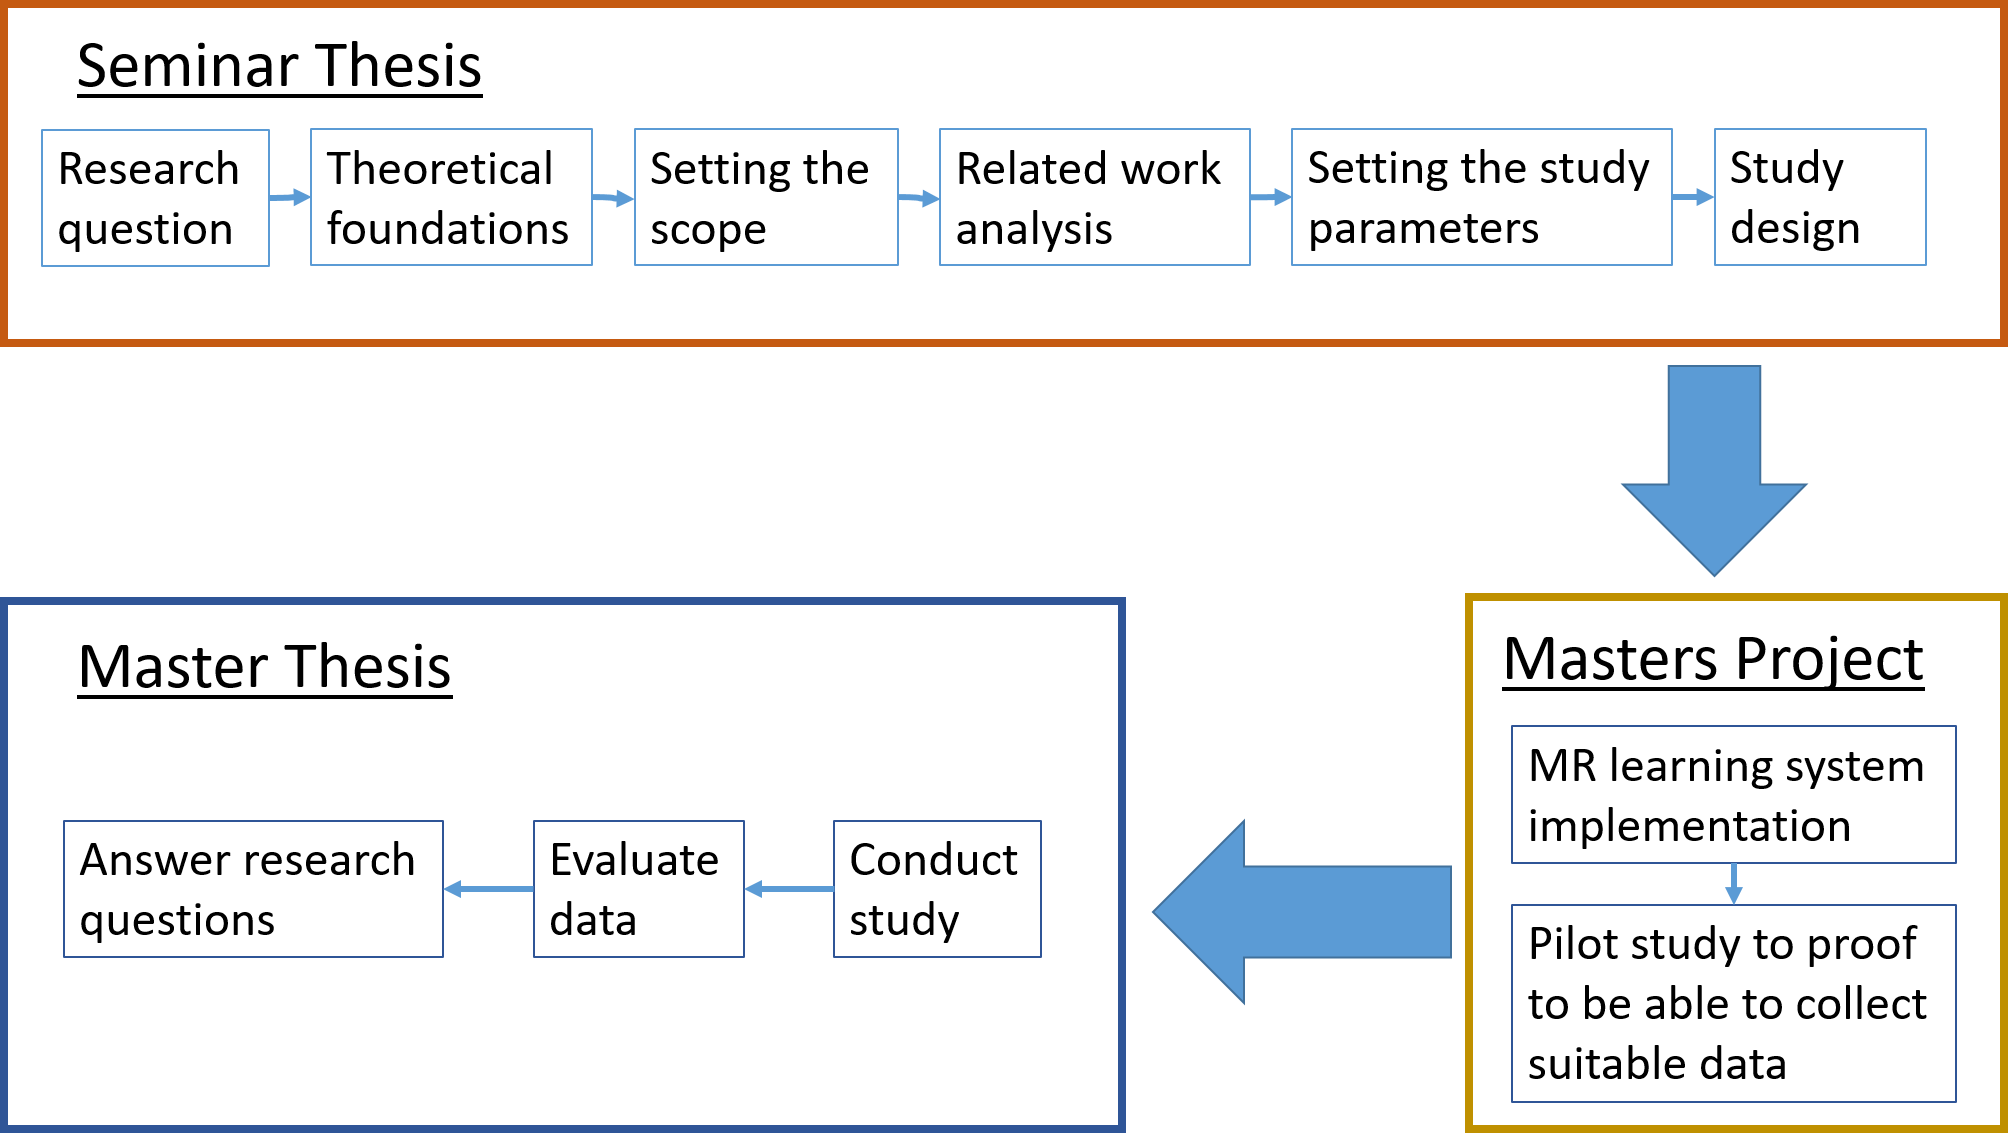
\includegraphics[width=1.0\textwidth]{img/overallProcess_new.png}
	\caption{Overall process of the masters thesis.}
	\label{fig:overallProcess}
\end{figure}\\

\begin{comment}
\begin{figure}
\centering
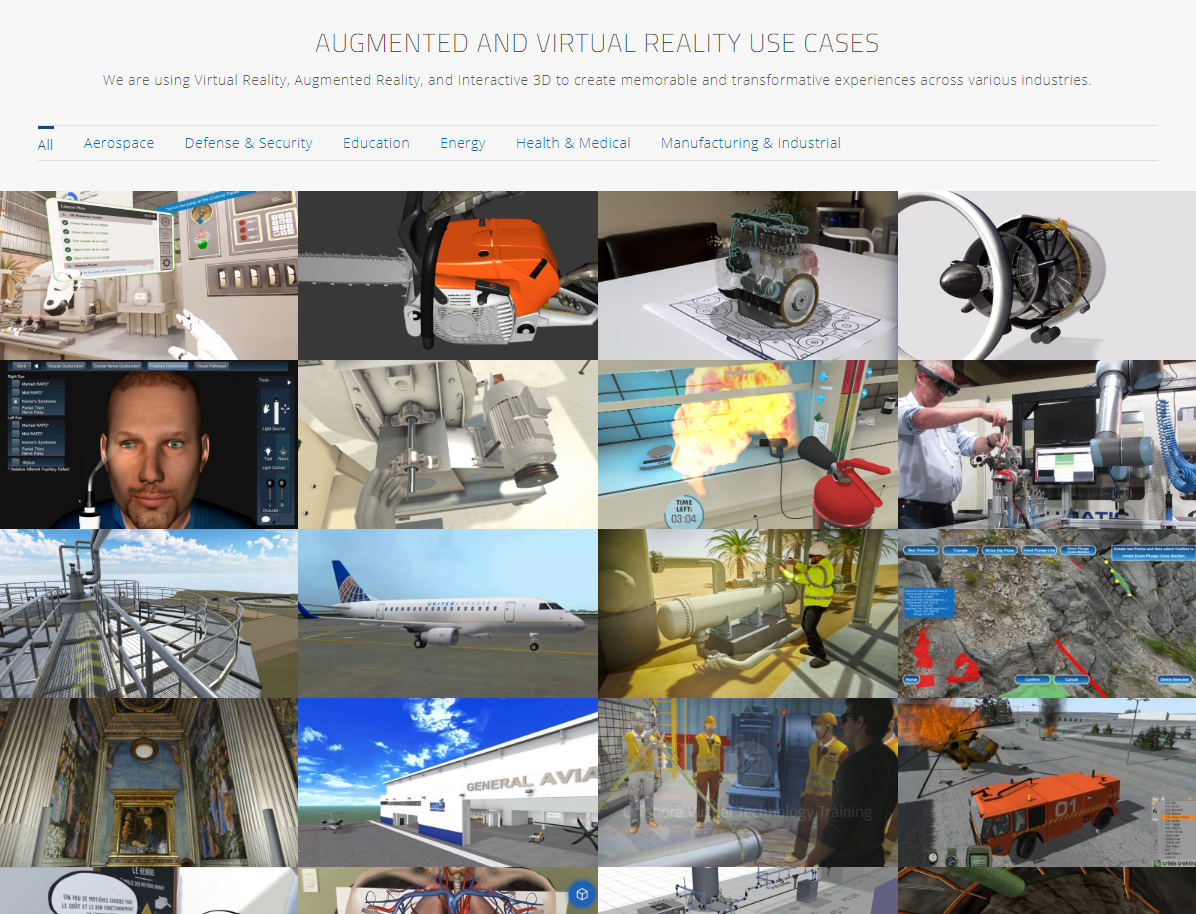
\includegraphics[width=1.0\textwidth]{img/eonreality.PNG}
\caption{Usecases by EONReality on their AVR plattform.  \hyperlink{https://www.eonreality.com/use-cases/}{eonreality.com/use-cases/} accessed 30.07.2019}
\label{fig:eonreality}
\end{figure}
\end{comment}
%Each of these aspects must be chosen wisely. In order to do so this seminar thesis will systematically go through every one of them. Chapter 3 sets the scope of the study and provides general knowledge about the domain. The following chapter 4 analyses the work of researchers and their systems, to find suitable components for the scope that has been set in chapter 4. Here, the remaining aspects are analysed from a more practical view and it is investigated how researchers decided about the aspects and why. Whenever a decision is made to be used in the proposed study design, a symbol on the side of the text can be found \markA. After all aspects are clear and reasoned, a study design is proposed in chapter 5. 

%first the theoretical background will be taken into consideration. It is mandatory to know how humans learn, classify, quantify and measure movements. In addition, recent MR hardware and tracking technology is investigated, a classification of perspectives is given and also a insight on MR itself. In this chapter we also set the res
%This seminar thesis will have a look at the grounding principles to define a system that lead to the guidelines in question. Therefore we first step into the theoretical background in the next chapter. We will investigate how people achieve motor skills, how to quantify and measure movements, what hardware techniques are suitable, perspectives and mixed reality. In the following chapter we analyse how other researchers used the theory to gain insights in Motor learing in VR. In the end we propose a study setting to that can be used to investigate on this topic.
%After this introduction, the scope of this thesis is given, where it is explained to what extend motor learning, MR, perspectives and other factors are considered. The following related work part will give an overview about other MR learning systems and also work about perspectives on avatars. From this work the measures, dependent and independent variables and tasks are derived. Taking the related work into consideration a study design is proposed in outlook section.